\chapter{Theory of Operation} 
\label{theory}  
\section{Nuclear Polarization}
In the presence of a magnetic field, spin-\half{} nuclei tend to align themselves along the axis of the field.  The polarization of the ensemble of particles is defined by 

\begin{eqnarray}
\label{eqn:polarization-definition}
\mathcal{P}=\frac{N_\uparrow-N_\downarrow}{N_\uparrow+N_\downarrow},
\end{eqnarray}

where $N_\downarrow$ ($N_\uparrow$) is the population of spins with $m_z$ equal to $-$\half{} (+\half).  For simplicity, the remainder of this section assumes particles of spin-\half{} unless otherwise stated.


\subsection{Zeeman Splitting}
\label{sec:zeemansplitting}

The effect of a constant magnetic field $B$ in the vicinity of an electron, i.e., a simple spin-\half{} particle, on its Hamiltonian is

\begin{eqnarray}
 H=-\vec{\mu}\cdot\vec{B},
\end{eqnarray}

where $\mu$ is the magnetic moment of the electron and the vector multiplication accounts for the direction of the field relative to the axis of the magnetic moment.  Taking both to be in the $z$-direction, we write the energy shift caused by this change in the Hamiltonian in terms of $\vec{\mu}=\mu\sigma_z$ as

\begin{eqnarray}
 \left<H\right>&\propto&\left<\mu B \sigma_z\right>\\
 &\propto&\mu B\left<\sigma_z\right> \\
 &\propto&B m_z,
\end{eqnarray}

where $m_z$ is the eigenvalue of the $\sigma_z$ operator and is positive (negative) when the spin is (anti-)aligned with the field.  For the spin-\half{} particle, the absolute value of $m_z$ is \half{}.

Figure \ref{fig:zeeman-splitting} shows the graph of this energy shift as a function of magnetic field.  The energy shift is a linear increase or decrease with field strength depending on whether the particle is aligned or anti-aligned.

\begin{figure}
 \centering
 
  \begin{tikzpicture}
    \begin{axis}[width=190pt,axis x line=left, axis y line=left, tick align=outside, xmin=0]
      \addplot+[mark=none,smooth] (\x,{\x});
      \addplot+[mark=none,smooth] (\x,{-\x});
    \end{axis}
  \end{tikzpicture}
  
  \caption{Zeeman splitting: TODO label plusorminus lines}
  \label{fig:zeeman-splitting}
\end{figure}
 

\subsection{Thermal Polarization Derivation}


A macroscopically sized target has $N$ particles, where $N$ is very large.  While any spin has exactly equal probability of being $\uparrow$ or $\downarrow$, it is not given that exactly half of $N$ are $\uparrow$.  This is easy to see when considering ten coins dropped on the ground: there is a $\approx$25\% chance that half of them will be heads and a $\approx$75\% chance of another outcome.


The relative odds of the system having $a$ particles $\uparrow$ to the system have $b$ particles $\uparrow$ is interesting.  To simplify notation, we give the name $M_x$ to number of ways of getting $x$ particles $\uparrow$ and call it the \textit{multiplicity} of getting $x$.  Now it becomes apparent that the probability $P_a$ of the system having $a$ spins $\uparrow$ is related to the probability $P_b$ of having $b$ spins $\uparrow$ is

\begin{eqnarray}
 \frac{P_a}{P_b} = \frac{M_a}{M_b},
\end{eqnarray}

since a higher multiplicity is associated with a higher probability for each state.

Using $S=k\ln M$ and other thermodynamic relationships (TODO come back and actually work all this out) we arrive at 

\begin{eqnarray}
 \frac{P_a}{P_b} = \frac{e^{-E_a/kT}}{e^{-E_b/kT}},
\end{eqnarray}

which is known as the Boltzmann factor that relates $P_a$ to $P_b$.  For the spin-\half{} system this gives us the ratios of populations

\begin{eqnarray}
 \frac{N_\downarrow}{N_\downarrow} = \frac{e^{E_\downarrow/kT}}{e^{E_\uparrow/kT}}.
\end{eqnarray}


We are now in position to rewrite the definition of polarization (Equation \ref{eqn:polarization-definition}) in terms of thermodynamic variables:

\begin{eqnarray}
 \mathcal{P}&=&\frac{N_\uparrow}{N_\uparrow+N_\downarrow}-\frac{N_\downarrow}{N_\uparrow+N_\downarrow} \\
 &=& \frac{1}{1+\frac{N_\downarrow}{N_\uparrow}}-\frac{1}{\frac{N_\uparrow}{N_\downarrow}+1} \\
 &=& \frac{1}{1+e^{-\Delta E/kT}}-\frac{1}{1+e^{\Delta E/kT}} \\
 &=& \tanh\left(\frac{\mu B}{kT}\right) \label{eqn:proton-polarization}
\end{eqnarray}

where $\Delta E\equiv E_\uparrow-E_\downarrow = 2 \mu B$, the typical difference in energy levels from a system undergoing Zeeman splitting.

\subsection{Thermal Polarization Values}

Equation \ref{eqn:proton-polarization} gives the degree of polarization for a proton in magnetic field $B$ and temperature $T$.  With modern cryogenic technology, it is relatively straightforward to cool a target sample to \SI{1}{\kelvin} and, using a superconducting solenoid magnet, magnetic fields as high as \SI{7}{\tesla}.

Plugging these numbers and the magnetic moment of the proton into the thermal polarization equation yields

\begin{eqnarray}
 \mathcal{P} &=& \tanh\left(\frac{\mu B}{kT}\right) \\
 &=& \tanh\left(\frac{(\SI{1.4E-26}{\joule/\tesla})(\SI{7}{\tesla})}{\left(\SI{1.3E-23}{\joule/\kelvin}\right)\left(\SI{1}{\kelvin}\right)}\right)\\
 &=&0.75\%.
\end{eqnarray}

The deuteron's polarization, which has a different dependence on $B$ and $T$ due to being a spin-1 system, can achieve thermal polarizations of

\begin{eqnarray}
 \mathcal{P} &=& \frac{4\tanh\frac{\mu B}{2kT}}{3+\tanh^2\frac{\mu B}{2kT}} \\
 &=& \frac{4\tanh\frac{(\SI{4.3E-27}{\joule/\tesla})(\SI{7}{\tesla})}{(2\SI{1.3E-23}{\joule/\kelvin})(\SI{1}{\kelvin})}}{3+\tanh^2\frac{(\SI{4.3E-27}{\joule/\tesla})(\SI{7}{\tesla})}{(2\SI{1.3E-23}{\joule/\kelvin})(\SI{1}{\kelvin})}}\\
 &=&0.02\%.
\end{eqnarray}

While the most modern systems can reach lower temperatures and higher fields, the marginal increase in polarization does not warrant dealing with practical issues of such systems.  For example, lowering $T$ from \SI{1}{\kelvin} to \SI{10}{\milli\kelvin}, a very difficult task, translates to a deuteron polarization of 1.9\%.


 \section{Dynamic Nuclear Polarization (DNP)}
 
If allowing the spin system to take on its thermal polarization distribution according to Maxwell-Boltzmann statistics is called \textit{static nuclear polarization}, then disturbing the equilibrium configuration to preferentially flip nuclear spins is called \textit{dynamic nuclear polarization}, or DNP.
 
\subsection{Solid State Effect}
One DNP process, called the Solid State Effect, uses microwave radiation to optically pump electron-proton pairs to energy states departing from thermal equilibrium (i.e., polarization states).  The relaxation time for the electron is much shorter than that of the proton, so the proton remains polarized while the electron is able to be paired with other protons for polarization.

The electrons available for optical pumping cannot be ordinary bound electrons, but must be so-called ``free radicals'', i.e., excess electrons present in the target material.  The two basic ways of introducing free radicals to the target sample are irradiation and chemical doping.  The method of irradiation involes putting the target in an ionizing beam line (TODO look up NIST specs for ionizing beam).  Chemical doping is adding a measured amount of a special chemical, sometimes a large molecular structure which hosts a single radical, to the target material before freezing into beads with liquid nitrogen.

The nuclei closest to the free radicals will couple more strongly and are more likely to flip during the solid state effect.  Nuclei-nuclei dipolar coupling then allows the polarized nucleus to transfer its polarization to another nucleus and become available for polarization by the free radical again.

\subsection{Equal Spin Temperature Theory}
Another DNP process, called Equal Spin Temperature, takes place when free-electron dopants are densely scattered throughout the nuclear sample.  When electron spin-spin interactions are no longer negligible, there exist distinct thermal reservoirs for the Zeeman and spin-spin interactions simultaneously.  Cooling just the spin-spin system, again with microwave radiation, puts the warmer nuclear reservoir in thermal contact with the cooled electron reservoir and subsequently cools down.

\subsection{Cross Effect}

The Cross Effect occurs when two electrons have differing spin-flip transition frequencies due to inhomogeneities in the target sample (TODO: learn more about what causes these inhomogeneities).  If the frequency difference is exactly equal to the spin-flip transition of a nearby nucleon, conservation of energy allows a simultaneous electron ``flip-flop'' with the flip of a nuclear spin.

\begin{figure}
 \centering
 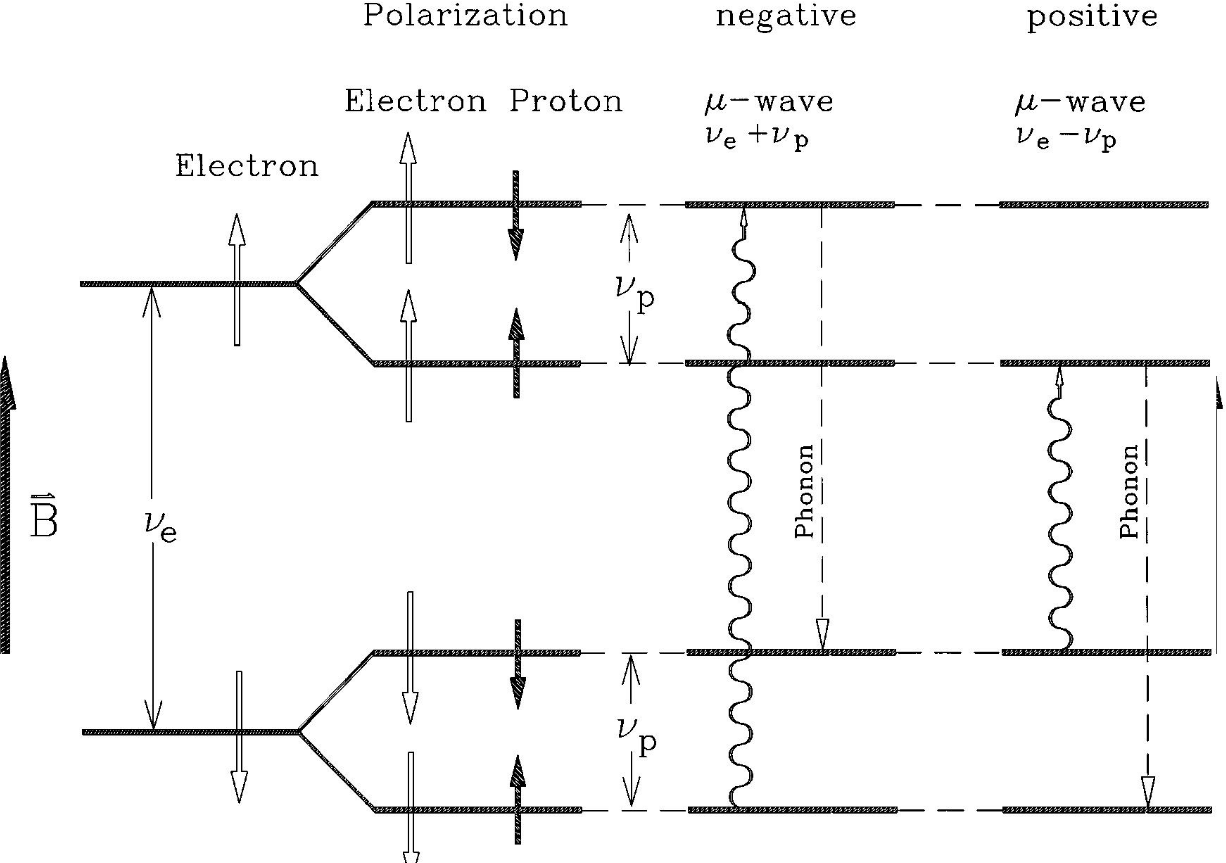
\includegraphics[scale=.25]{img/dnp.png}
 % dnp.png: 1226x863 pixel, 72dpi, 43.25x30.44 cm, bb=0 0 1226 863
 \caption{DNP diagram \cite{dnpdiagram}.  The white arrows are electron polarization and the black arrows are proton polarization.  Microwaves at a frequency difference $\nu_e\pm\nu_p$ flip the spins of both particles, and the electron's superior lattice coupling ensures it will flip back before the proton.}
 \label{fig:dnp-diagram}
\end{figure}


The microwave frequency can either be the sum of the proton and electron splitting frequency or the difference, depending on whether the nucleons are to be aligned with or against the magnetic field. 
\section{NMR}

Nuclear Magnetic Resonance (NMR) is the method we use to measure the polarization of the target material.  Essentially, a coil in the immediate vicinity of the target acts as the inductor in an LCR circuit, the inductance of which changes as a function of the magnetic susceptibility of the nuclei in the coil.  Since the magnetic susceptibility and polarization are related, the resonance frequency of the LCR circuit tell us information about the polarization of the target material\cite{qmeterbook}. 

\subsection{Liverpool Q-Meter}

The Q-Meter houses the capacitor and resistor for the LCR circuit, as well as detectors that transform the signal into usable data representing polarization\footnote{Much of this section is from PTGroup's Lab Overview\cite{laboverview}}.  The Q-Meter is entirely encased in gold-plated brass to keep out RF noise from the lab, and all connectors and cables carrying RF signals that connect to the Q-Meter must also be similarly shielded.

\subsubsection{LCR Circuit}
\label{lcr}
The \textit{Liverpool NMR Module} is a system for measuring the polarization of polarized nuclei using Q-Meter measurements of their resonant frequency.  It uses an LCR circuit with the polarized material contained in the inductor. The resonant frequency of the circuit is calibrated to be the same as the magnetic resonant frequency of the material, given the value of the base magnetic field. The polarized material affects the inductance of the circuit and therefore produces a change in the quality factor, $Q$, as measured by a device called a Q-Meter, as well as impedance. This change is measured by applying a frequency swept RF voltage to the tuned circuit and detecting the change in impedance as a change in current or voltage. The different elements of the Liverpool Module are arranged in the \textit{Q-Circuit} (Figure \ref{NMR-q-circuit-schematic}).\\

\begin{figure}
	\centering
	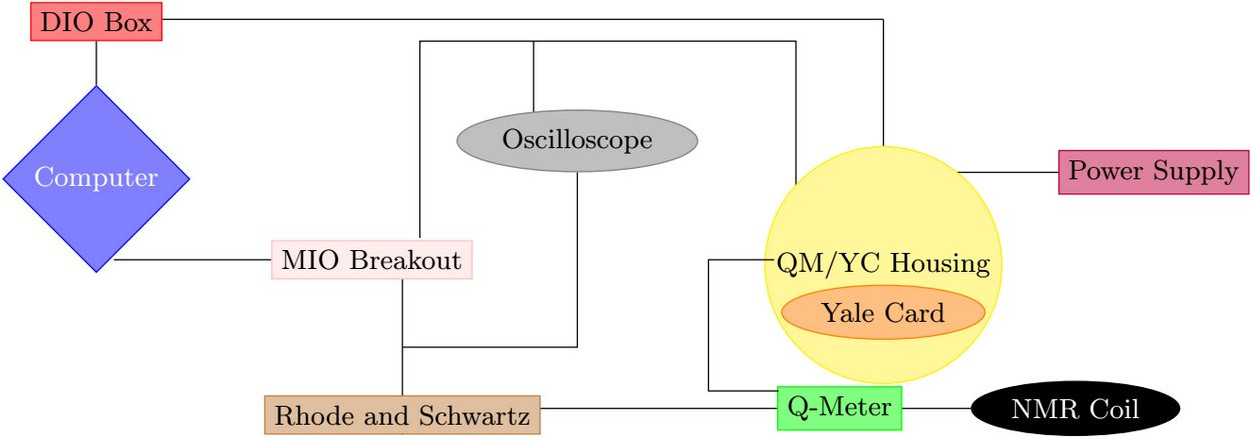
\includegraphics[width=4in,angle=0]{img/NMR-q-circuit-schematic.jpg}
	\caption{Q-circuit schematic}
	\label{NMR-q-circuit-schematic}
\end{figure}
\subsubsection{Q-Curve}
A plot of the RS frequency on the x-axis and the max signal (in volts) seen by the scope is called a \textit{Q-Curve} (Figure \ref{qcurve-tikz}).

\begin{figure}
  \centering
  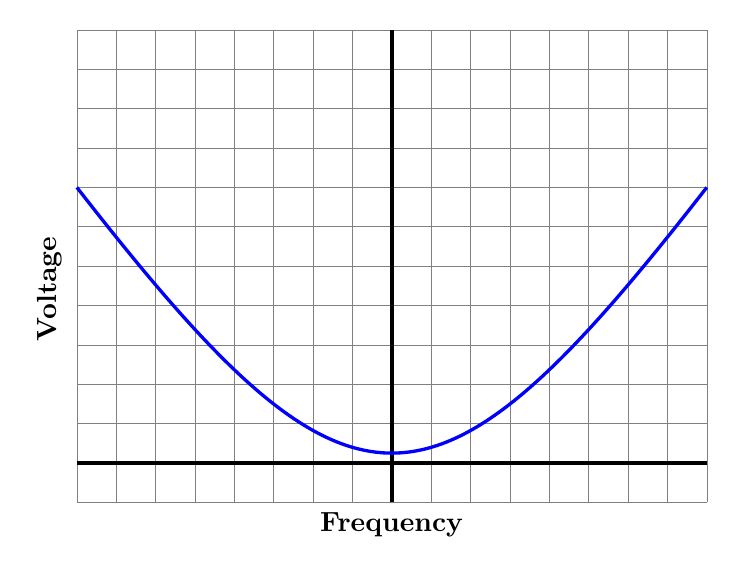
\begin{tikzpicture}
    \draw [step=.5cm, draw=gray, very thin](-4,-.5) grid (4,5.5);
    \draw [ultra thick] (0,-.5)--(0,5.5);
    \draw[ultra thick] (-4,0)--(4,0);
    \draw[very thick,draw=blue] (-4,3.5)..controls(-.5,-1) and (.5,-1)..(4,3.5);
    \draw (-4,3) node [left=10pt, rotate=90]{\textbf{Voltage}};
    \draw(0,-.5) node [anchor=north]{\textbf{Frequency}};
  \end{tikzpicture}
  \caption{A Q-Curve plot with RS frequency on the X-axis and scope (detector) signal on the Y-axis.  Compare the left half of this plot with the above triple plot (as RS frequency goes down, scope signal goes up).}
  \label{qcurve-tikz}
\end{figure}

This curve can be shown on the scope's XY mode by plugging the RS's input to channel 1 and the diode detector on channel 2. A Q-Curve is referred to as \textit{tuned} when the central frequency of the RS sweep is at the center of the Q-Curve.  Since the central frequency is fixed, this is achieved by adjusting L and C of the circuit so the LCR resonance equals the desired frequency. 


A Q-Curve tuned to the resonance frequency of a polarized target has a very special quality.  When something is placed inside the inductor of the circuit, like an actual polarized target or a ``dummy'' oscillator chip that absorbs EM radiation at the resonance frequency, we see an aberration (TODO: replace Figure \ref{NMR-qcurve-scope} with one that has an actual aberration) on the scope where the x-axis marks resonance (Figure \ref{NMR-qcurve-scope}).  The more polarized a target is, the larger the aberration will be.\\

\begin{figure}
  \centering
  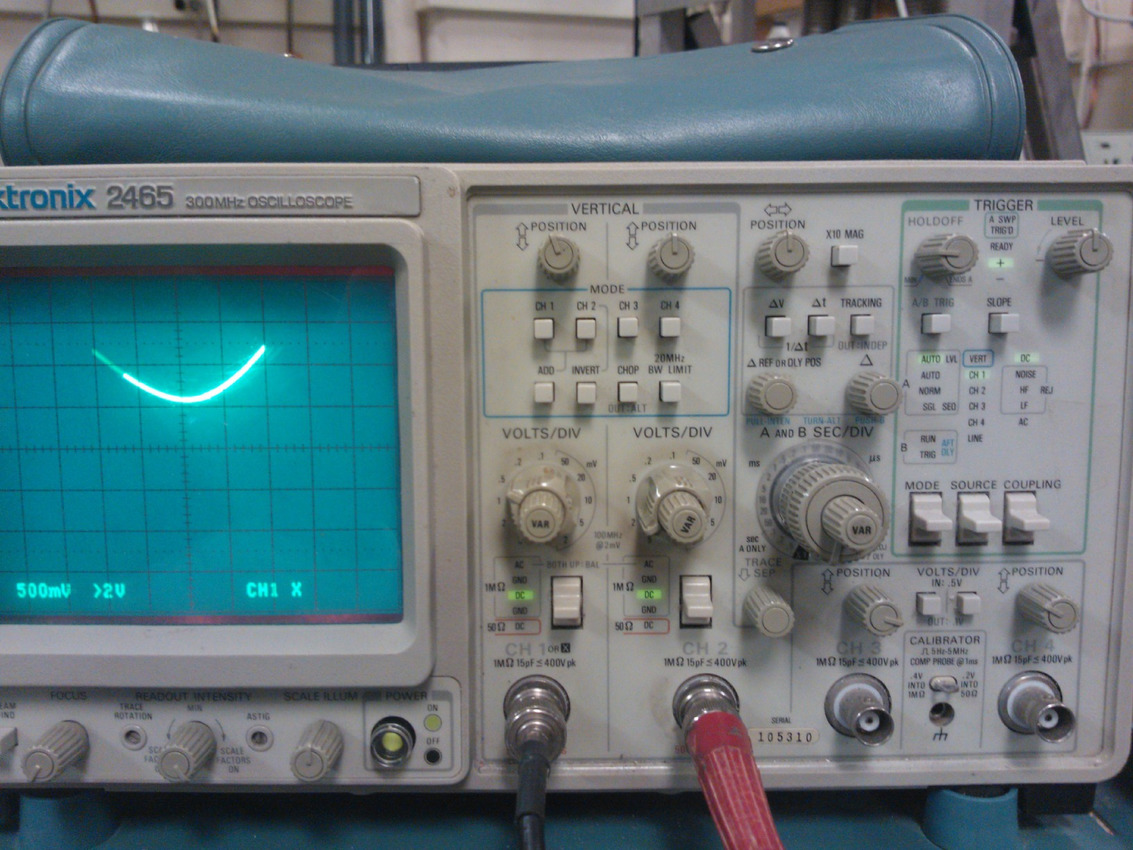
\includegraphics[width=4in,angle=0]{img/NMR-qcurve-scope.jpg}
  \caption{The Q-Curve as it is seen on the oscilloscope}
  \label{NMR-qcurve-scope}
\end{figure}

The nature of the aberration is dependent on the nuclear species, the molecular structure the nucleus is in (usually an ammonia or alcohol) and some other factors.  In all cases, the aberration arises because the resonance frequency corresponds to a photon of energy equal to the nuclear Zeeman splitting that stimulates emission/absorption from the target material (see Section \ref{sec:zeemansplitting}).\\

The Q-Curve without the aberration is subtracted from the Q-Curve with the aberration (called a \textit{background subtraction}) and what remains is a bump with an area proportional to the polarization of the target material. In this way, an LCR circuit is used in the NMR setup to measure nuclear polarization.\\ 

\subsubsection{Diode Detector}
The output of the LCR circuit is a sine wave of the same frequency as the RS output.  A diode detector is basically a full wave rectifier that smoothes out the magnitude of the resulting waveform (Figure \ref{diode}).

\begin{figure}
  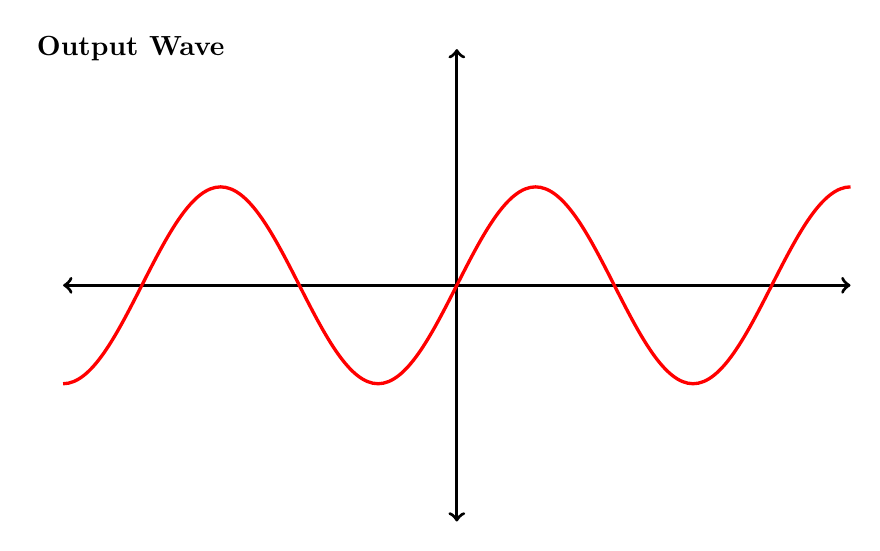
\begin{tikzpicture}
    \draw[very thick,<->] (0,-3)--(0,3) node[left=80pt]{\textbf{Output Wave}};
    \draw[very thick,<->](-5,0)--(5,0);
    \draw[very thick,red](-5,-1.25)cos    (-4,0)sin(-3,1.25)cos(-2,0)sin(-1,-1.25)cos(0,0)sin(1,1.25)cos(2,0)sin(3,-1.25)cos(4,0)sin(5,1.25);
  \end{tikzpicture}
  \vspace{6mm}
  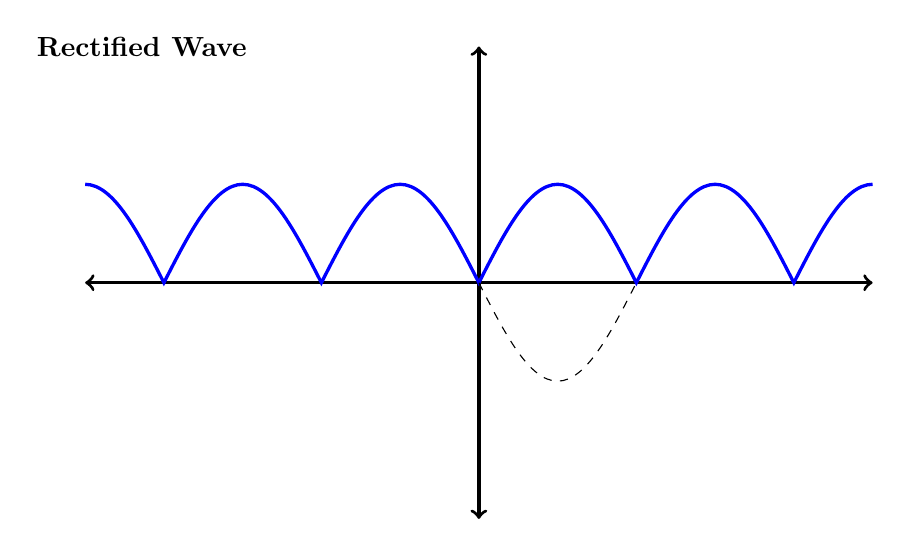
\begin{tikzpicture}
    \draw[very thick,<->] (0,-3)--(0,3) node[left=80pt]{\textbf{Rectified Wave}};
    \draw[very thick,<->](-5,0)--(5,0);
    \draw[very thick,blue](-5,1.25)cos    (-4,0)sin(-3,1.25)cos(-2,0)sin(-1,1.25)cos(0,0)sin(1,1.25)cos(2,0)sin(3,1.25)cos(4,0)sin(5,1.25);
    \draw[dashed](0,0)sin(1,-1.25)cos(2,0);
  \end{tikzpicture}
  \caption{The output of the LCR circuit (top) and that same output rectified by a diode detector (bottom)}
  \label{diode}
\end{figure}

The output can be thought of as a DC voltage comparable to the peak signal from the LCR circuit. Tuning always begins by looking at the diode because it makes finding the correct $\lambda$/2 cable length and Q-Meter capacitance simpler.

\subsubsection{Phase Detector and Phase Cable}
Once a signal is seen with the diode detector, we switch to a more sensitive detector built into the Q-Meter. The phase detector has a core component called a balanced ring modulator (BRM) that takes two inputs, the LCR signal and the RS signal, and provides one output, an phase-dependent signal that indicates target polarization.\\

Generally, a BRM multiplies the two input signals and outputs a signal proportional to the phase difference between them.  When no polarized target is present, the relative phase between inputs is adjusted to zero by adding electrical path length with a so-called phase cable.  When the phase difference is set to zero, the BRM output is proportional to the real part of the LCR signal. For this reason, the phase detector is also sometimes called a ``real part'' detector. The phase cable is adjusted just like the $\lambda$/2 cable, except it is shorter and both ends are connected to the Q-Meter (see PTGroup's “Q-Meter Tune'' document for tuning details).\\

\subsection{$\lambda$/2 Cable}

\begin{figure}
  \centering
  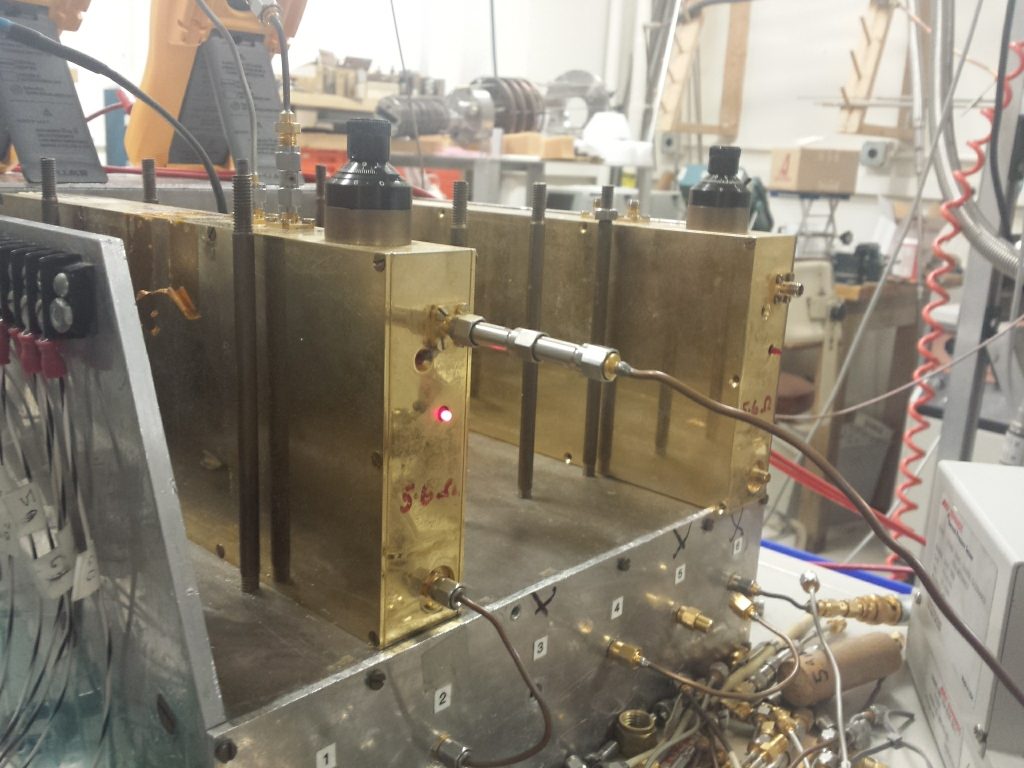
\includegraphics[width=4in, angle=0]{img/NMR-lambda-cable.jpg}
  \caption{A $\lambda$/2 cable attached to the Q-Meter}
  \label{NMR-lambda-cable}
\end{figure}
Because polarization requires that the target material be kept at a very low temperature and the lab's electronics are inoperable at such temperatures, the inductor coil must be coupled to the circuit by use of cables of length comparable to the wavelength of the RF (that is, $\lambda$).  In this way, the impedance due to the inductor is the same as it would be if there was no cable attachment. \\

If the electrical path between the Q-Meter and coil had a length different than n$\lambda$/2, the Q-Meter would see an (input-) impedance larger than the coil's actual (load-) impedance. For our purposes, the load impedance is the actual resistance of the NMR coil, and the input impedance is the resistance the coil appears to be from the Q-Meter.  If the Q-Meter is some length $l$ from the coil, then the input impedance it sees is given by

\begin{center}
  $Z_{\textrm{input}} = K\frac{Z_L+K\tanh(i2\pi l/\lambda)}{K+Z_L\tanh(i2\pi l/\lambda)}$
\end{center}
where $K$ is a constant characteristic of the cable, called its \textit{characteristic impedance}.  Clearly, this is at a minimum when the Q-Meter is a multiple of half a wavelength, which is when the input impedance equals the load impedance.\\

The above is a simplification: the cables are actually lossy so the given equation has an attenuation component, the velocity of light in the cable needs to be taken into account when determining $l$, fridge temperature and phase-transition temperatures of materials within the cables can play a role, etc.  However, these effects are easily corrected for or otherwise tend to be negligible.\\

In the lab, the length $l$ is already at some minimum value because of the finite electrical path inside the Q-Meter and inside the fridge.  In addition to that unchangable length, the Q-Meter is connected to the fridge with a $\lambda$/2 cable. $l$ is adjusted by adding or removing length to this cable, which can be tedious since there is no continuous variable adjustment.  Most cables are female-female so must therefore be mated with a male-male barrel, and the RF connectors should be tightened with a special torque-limiting wrench to ensure sufficient electrical contact. Suboptimal connections between the constituent $\lambda$/2 cable components leads to unpredictable and often irrepeatable signals on the scope.  Additionally, all cables are ``semi-rigid'' meaning they have copper shields which make them difficult to bend. The biggest difficulty trying to get the right $\lambda$/2-cable length tends to be finding the right combination of cables that sum to the desired length.\\


%\subsection{DAQ}

%\subsection{PDP}

\section{Frozen Spin} 
 
 The target is polarized in a 2.5 T field, called the polarizing field, generated from a large, super-conducting magnet (TODO photo).  Without this polarizing field, the target immediately loses all polarization due to lack of a quantization axis.  Physically, the magnet obstructs the path between the target and detectors, greatly reducing the solid angle available. We wish to employ a method of maintaining target polarization without the polarizing magnet in the way.  The method of choice is Hifrost's namesake frozen spin method.
 
 
 A 0.5 T field, generated from an internal superconducting coil (TODO photo), is ramped up while the target is at maximum polarization.  At dilution temperatures, this smaller field, called the holding field, sufficiently maintains nuclear polarization while the polarizing magnet is removed and the detector is placed around the target (TODO diagram). 
 
 

\section{Refrigerator} 
Since the polarization goes like the inverse of temperature, colder environments make for better polarized targets.  In our case, we use a dilution refrigerator, one that mixes the two isotopes \het{} and \hef{} for cooling, to reach target temperatures below 0.1 K.


Also, in the case of the frozen spin target, the dilution frigerator is our only recourse to maintain polarization without a large magnet for an amount of time suitable for a nuclear physics experiment.

\subsection{\hef{}Cooling (Evaporator and Separator)}

\subsection{Dilution}

The dilution refrigerator principle relies on the splitting of a \het/\hef{} mixture into two distinct phases, a \het{} concentrated phase and a \het{} dilute phase.  The area labeled ``Two-phase region'' in Figure \ref{fig:dilutiondiagram} illustrates which mixtures, characterized by \het{} concentration, are inaccessible at which temperatures.  Since two distinct phases in thermal contact are always in or striving for thermodynamic equilibrium, changing the concentration of the dilute phase (by pumping \het{} out of it) will cause atoms from the concentrated phase to cross the phase boundary to restore balance.  Since the heat change of mixing (enthalpy difference between the dilute phase and concentrated phase) is positive, the \het{} crossing the phase boundary must absorb energy from the surrounding environment, which it does in the form of heat.\cite{hocktechniques}

\begin{figure}
 \centering
 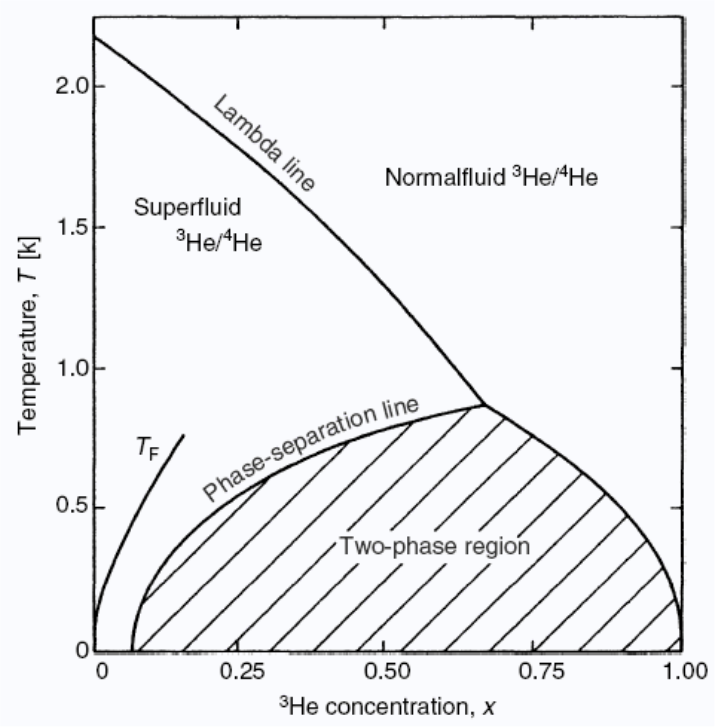
\includegraphics[scale=.45]{img/dilutiondiagram.png}
 % dilutiondiagram.png: 715x727 pixel, 72dpi, 25.22x25.64 cm, bb=0 0 715 727
 \caption{The famous diagram that shows the splitting of two distinct phases of $\het$-$\hef$ mixture. \cite{dilutiondiagram}}
 \label{fig:dilutiondiagram}
\end{figure}
 
